%%%%%%%%%%%%%%%%%%%%%%%%%%%%%%%%%%%%%%%%%
% Beamer Presentation
% LaTeX Template
% Version 1.0 (10/11/12)
%
% This template has been downloaded from:
% http://www.LaTeXTemplates.com
%
% License:
% CC BY-NC-SA 3.0 (http://creativecommons.org/licenses/by-nc-sa/3.0/)
%
%%%%%%%%%%%%%%%%%%%%%%%%%%%%%%%%%%%%%%%%%

%----------------------------------------------------------------------------------------
%	PACKAGES AND THEMES
%----------------------------------------------------------------------------------------

\documentclass{beamer}

\mode<presentation> {

% The Beamer class comes with a number of default slide themes
% which change the colors and layouts of slides. Below this is a list
% of all the themes, uncomment each in turn to see what they look like.

%\usetheme{default}
%\usetheme{AnnArbor}
%\usetheme{Antibes}
%\usetheme{Bergen}
%\usetheme{Berkeley}
%\usetheme{Berlin}
%\usetheme{Boadilla}
%\usetheme{CambridgeUS}
%\usetheme{Copenhagen}
%\usetheme{Darmstadt}
%\usetheme{Dresden}
%\usetheme{Frankfurt}
%\usetheme{Goettingen}
%\usetheme{Hannover}
%\usetheme{Ilmenau}
%\usetheme{JuanLesPins}
%\usetheme{Luebeck}
%\usetheme{Madrid}
%\usetheme{Malmoe}
%\usetheme{Marburg}
%\usetheme{Montpellier}
%\usetheme{PaloAlto}
%\usetheme{Pittsburgh}
%\usetheme{Rochester}
%\usetheme{Singapore}
%\usetheme{Szeged}
\usetheme{Warsaw}

% As well as themes, the Beamer class has a number of color themes
% for any slide theme. Uncomment each of these in turn to see how it
% changes the colors of your current slide theme.

%\usecolortheme{albatross}
%\usecolortheme{beaver}
%\usecolortheme{beetle}
%\usecolortheme{crane}
%\usecolortheme{dolphin}
%\usecolortheme{dove}
%\usecolortheme{fly}
%\usecolortheme{lily}
%\usecolortheme{orchid}
%\usecolortheme{rose}
%\usecolortheme{seagull}
%\usecolortheme{seahorse}
%\usecolortheme{whale}
%\usecolortheme{wolverine}

%\setbeamertemplate{footline} % To remove the footer line in all slides uncomment this line
%\setbeamertemplate{footline}[page number] % To replace the footer line in all slides with a simple slide count uncomment this line

%\setbeamertemplate{navigation symbols}{} % To remove the navigation symbols from the bottom of all slides uncomment this line
}

\usepackage{graphicx, verbatim, lmodern} % Allows including images
\usepackage{booktabs} % Allows the use of \toprule, \midrule and \bottomrule in tables

%----------------------------------------------------------------------------------------
%	TITLE PAGE
%----------------------------------------------------------------------------------------

\title[Euler paths and circuits on digraphs and genome sequencing]{Euler paths and circuits on digraphs and genome sequencing} % The short title appears at the bottom of every slide, the full title is only on the title page

\author{Nilay Bhatt} % Your name
\institute[CCSU] % Your institution as it will appear on the bottom of every slide, may be shorthand to save space
{
Central Connecticut State University \\ % Your institution for the title page
\medskip
\textit{nilaybhatt@my.ccsu.edu} % Your email address
}
\date{\today} % Date, can be changed to a custom date

\begin{document}

\begin{frame}	
\titlepage % Print the title page as the first slide
\end{frame}

\begin{frame}
\frametitle{Overview} % Table of contents slide, comment this block out to remove it
\tableofcontents % Throughout your presentation, if you choose to use \section{} and \subsection{} commands, these will automatically be printed on this slide as an overview of your presentation
\end{frame}

%----------------------------------------------------------------------------------------
%	PRESENTATION SLIDES
%----------------------------------------------------------------------------------------

%------------------------------------------------
\section{Definitions} 
\begin{frame}
\frametitle{Definitions}
\begin{definition}[Graph]
A \textbf{graph} $G$ consists of a non-empty finite set $V(G)$ of elements called \textbf{vertices},
and a finite `family'  $ E(G)$ of unordered pairs of (not necessarily distinct) elements
of $V(G)$ called \textbf{edges}.
\end{definition}
\pause
\begin{itemize}
\item Too formal? Think of a graph as a bunch of tennis balls connected with a thread.
\end{itemize}
\pause
\begin{definition}[Digraph]
A \textbf{digraph} $G$ consists of a non-empty finite set $V(G)$ of elements called \textbf{vertices},
and a finite `family'  $E(G)$ of ordered pairs of distinct elements of $V(G)$ called \textbf{directed edges}.
\end{definition}
\pause
\begin{itemize}
\item NYC grid with all the streets being one-way, which then restricts our movement on the graph.
\end{itemize}
\end{frame}

%------------------------------------------------

%\subsection{Subsection Example} % A subsection can be created just before a set of slides with a common theme to further break down your presentation into chunks

\begin{frame}
\frametitle{Graphs and Digraphs}
\begin{figure}[h]
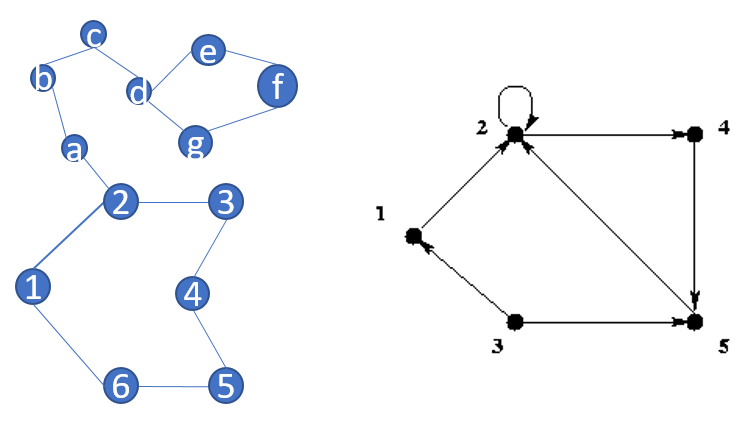
\includegraphics[width=\textwidth]{graphs.png}
\end{figure}
\end{frame}

%------------------------------------------------
\section{Eulerian Graphs}
\begin{frame}
\frametitle{Euler Paths vs. Circuits}
\begin{definition}[Euler Path]
 An \textbf{Euler path} on a graph $G$ is a special walk that uses each edge exactly once, and it starts and ends at \textbf{different} vertices.
\end{definition}
\begin{definition}[Euler Circuit]
 An \textbf{Euler circuit} on a graph $G$ is a walk that uses each edge exactly once, and it starts and ends at the \textbf{same} vertex.
\end{definition}
\end{frame}

%------------------------------------------------
\begin{comment}
\begin{frame}
\frametitle{Euler Path}
\begin{figure}[h]
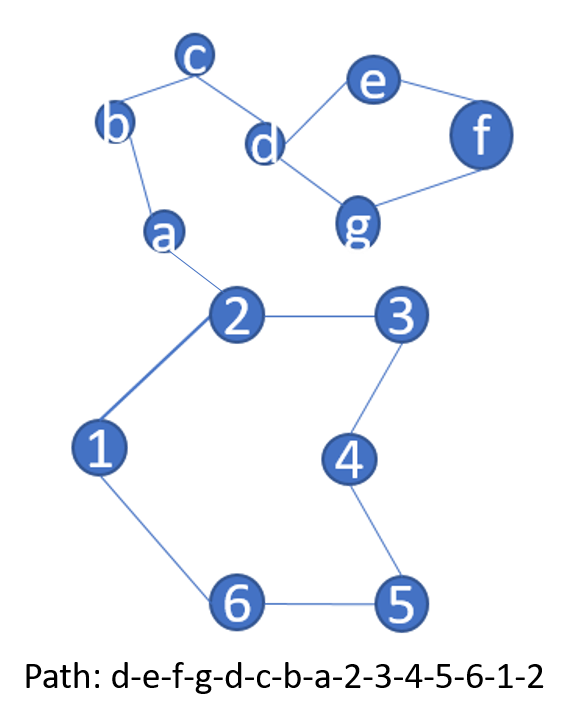
\includegraphics[scale = 0.3]{path.png}
\end{figure}
\end{frame}

%------------------------------------------------

\begin{frame}
\frametitle{Euler Circuit}
\begin{figure}[h]
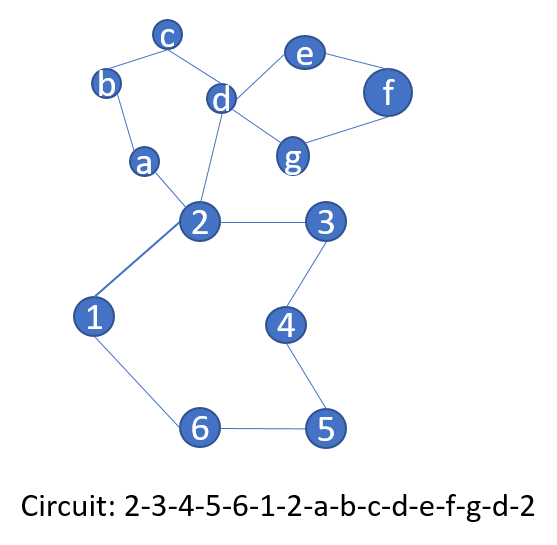
\includegraphics[scale = 0.4]{circuit.png}
\end{figure}
\end{frame}
\end{comment}

%------------------------------------------------


\begin{frame}
\frametitle{Criterion for an Euler path or circuit on a graph}
\begin{block}{Euler Path}
A given graph $G$ has an Euler path if and only if the graph is connected and \textbf{all but 2 vertices in the graph are of odd degree.}
\end{block}
\pause
\begin{itemize}
\item What extra condition do you think we need to add for a digraph to have an Euler path?
\end{itemize}
\end{frame}

%------------------------------------------------

\begin{frame}
\frametitle{Can we find an Euler Path?}
\begin{figure}[h]
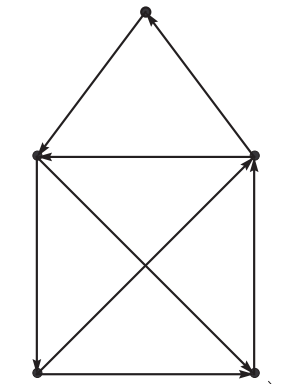
\includegraphics[scale = 0.628]{pathdi.png}
\end{figure}
\end{frame}

%------------------------------------------------

\begin{frame}
\frametitle{YES WE CAN!}
\begin{figure}[h]
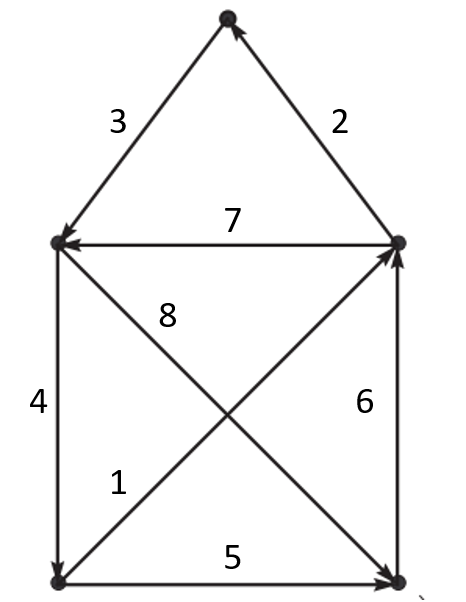
\includegraphics[scale = 0.4]{pathdisol.png}
\end{figure}
\end{frame}

%------------------------------------------------

\begin{frame}
\frametitle{Criterion for an Euler path on a digraph}
\begin{block}{Euler Path}
A given graph $G$ has an Euler path if and only if the graph is connected and \textbf{all but 2 vertices in the graph are of odd degree.}
\end{block}

\begin{block}{Euler Path on a digraph}
A digraph $D_g$ has an Euler path iff
\begin{itemize}

\item The graph is connected 
\item All but 2 vertices in the graph are of odd degree
\item \textbf{the \textbf{$|$indegree $-$ outdegree$|$ = 1} for those two odd vertices in $D_g$.}

\end{itemize}
\end{block}
\end{frame}

%------------------------------------------------

\begin{frame}
\frametitle{Criterion for an Euler circuit on a digraph}
\begin{block}{Euler Circuit}
A graph $G$ has an Euler circuit if and only if $G$ is connected and all the vertices are of \textbf{even degree} . 
\end{block}
\pause
\begin{itemize}
\item What extra condition do you think will be needed on a digraph for it to have an Euler circuit?
\end{itemize}
\end{frame}

%------------------------------------------------

\begin{frame}
\frametitle{Euler Circuit on digraph}
\begin{figure}[h]
\includegraphics[scale = 0.8]{eulerdi.jpg}
\end{figure}
\end{frame}

%------------------------------------------------

\begin{frame}
\frametitle{Criterion for an Euler circuit on a digraph}
\begin{block}{Euler Circuit}
A graph $G$ has an Euler circuit if and only if $G$ is connected and all the vertices are of \textbf{even degree} . 
\end{block}
\begin{block}{Euler circuit on a digraph}
A graph $D_g$ has an Euler circuit if and only if $D_g$ is connected and all the vertices are of even degree and the \textbf{indegree = outdegree}
for all vertices.
\end{block}
\begin{itemize}
\item A formal proof done as part of the final project in Senior Seminar (Spring 2017)
\end{itemize}
\end{frame}

%------------------------------------------------

\begin{frame}
\frametitle{How to find an Euler path and/or circuit on a graph?}
Recall: For an Euler Path all but 2 vertices must be of odd degree and to have an Euler circuit has all vertices must be of even degree.
\pause
\\  While traversing (removing edges once traversed), if removal of a single edge from the remaining connected graph makes it disconnected then such an edge is called a \textbf{bridge}.

\begin{itemize}

\item To create an Euler path, start at either of the odd vertices.
\pause
\item Follow edges one at a time and if you come across a bridge and a non-bridge: Always choose Non-bridge
\end{itemize}
\pause
This is called \textbf{Fleury's Algorithm}
\end{frame}

%------------------------------------------------


\begin{frame}
\frametitle{Find an Euler Path?}
\begin{figure}[h]
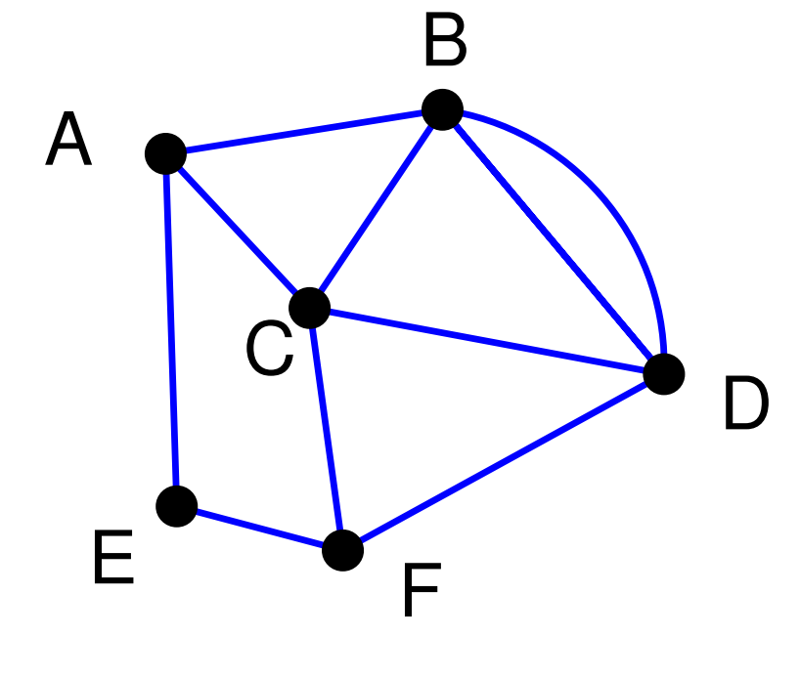
\includegraphics[scale = 0.4]{path2.png}
\end{figure}
\end{frame}

%------------------------------------------------

\begin{frame}
\frametitle{What's next?}
This is cool, but for all the applied mathematicians in the room and computer engineers like me the question becomes:\\ 
\textbf{\begin{center}
How does that help me?
\end{center}}
\end{frame}

%------------------------------------------------

%------------------------------------------------
%------------------------------------------------
\section{Applications}
%------------------------------------------------
%------------------------------------------------

%------------------------------------------------

\begin{frame}
\frametitle{Applications}
\begin{enumerate}
\item Mathematical modeling
\item {\color{red}\textbf{DNA fragment reconstruction}}
\item Postman problem
\item Traveling salesman problem

\item many more ....
\end{enumerate}
\end{frame}

%------------------------------------------------

\begin{frame}
\frametitle{Genome Sequencing}
\textbf{DNA}
\begin{columns}[c]

\column{.45\textwidth}

\begin{figure}[h]
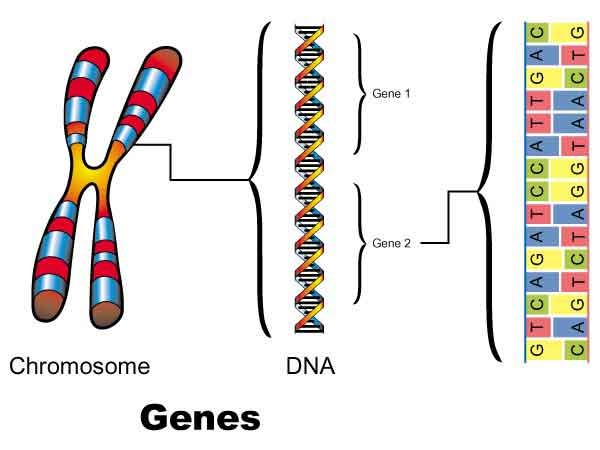
\includegraphics[scale = 0.35]{dna.jpg}
\end{figure}

\column{.45\textwidth}


\begin{itemize}
\item Protein that stores the genetic information of a living organism
\pause
\item Four components to it: A,T,G,C. A connects to T and G connects to C
\pause
\item Fragments of DNA are used in genetic research and discovery
%\item If any cancer is genetically triggered, or how hereditary diabetes is and how mutations occur
\item Strings of such {\color{red}ATGC} pairs have this information stored in them	
\end{itemize}


\end{columns}
\end{frame}

%------------------------------------------------

\begin{frame}
\frametitle{Genome Sequencing}
\begin{itemize}
\item Reads are taken of a known DNA strand (Sanger, 1977)
\item They vary in size from 30-800 nucleotides
\item Reads are taken in an overlapping form
\item Reconstructing the specific genome with the overlapping to create a superstring is NP-complete
\end{itemize}
\end{frame}

%------------------------------------------------

\begin{frame}
\frametitle{Shortest Super String Problem}
Problem: \textbf{Given a set of strings, find a shortest string that contains all of them} - NP Complete
\begin{figure}[h]
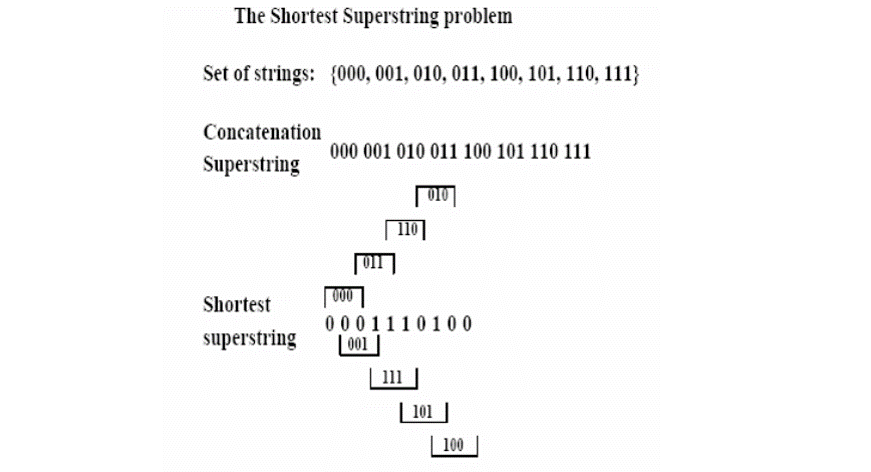
\includegraphics[scale = 0.4]{ssexample.png}
\end{figure}
\end{frame}

%------------------------------------------------

\begin{frame}
\frametitle{De Bruijn Sequence Approach}
\begin{itemize}
\item Given a string, split it into $k-mers$
\pause
\item Then split each $k-mers$ into $k-1-mer$
\pause
\item Now assign the two $k-1-mers$ as vertices and the $k-mer$ as the name of the directed edge
\pause
\item Consolidate the duplicate edges (collapse them, while conserving the directed edges
\pause
\item The final directed Euler Path is the super string
\end{itemize}
\end{frame}

%------------------------------------------------

\begin{frame}
\frametitle{What is a $k-mer$ composition of a given genome string}

Given a string : \textbf{\textit{TAATGCCATGGGATGTT}}, what is a 3-mer composition?\\
= $\{TAA, AAT, ATG, TGC, GCC, CCA, CAT,$\\ $ ATG, TGG, GGG, GGA, GAT, ATG, TGT, GTT\}$
\begin{itemize}
\item We use these 3-mers as labels of directed edges.
\pause
\begin{figure}[h]
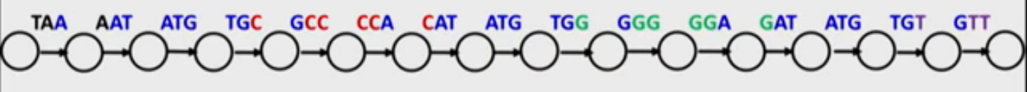
\includegraphics[scale = 0.4]{3mer.png}
\end{figure}
\pause
\begin{figure}[h]
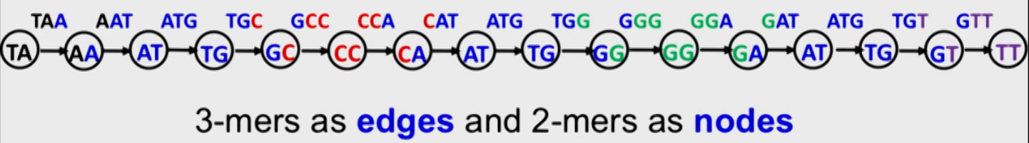
\includegraphics[scale = 0.4]{3mer2mer.png}
\end{figure}
\end{itemize}
\end{frame}

%------------------------------------------------

\begin{frame}
\frametitle{Collapsing like vertices on itself}
\begin{figure}[h]
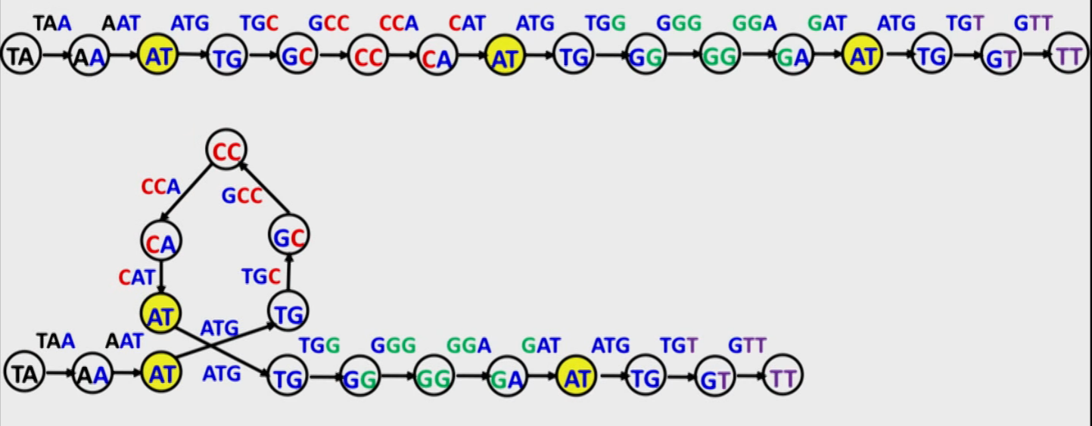
\includegraphics[scale = 0.4]{gluing.png}
\end{figure}
\end{frame}

%------------------------------------------------

\begin{frame}
\frametitle{Collapsing like vertices on itself}
\begin{figure}[h]
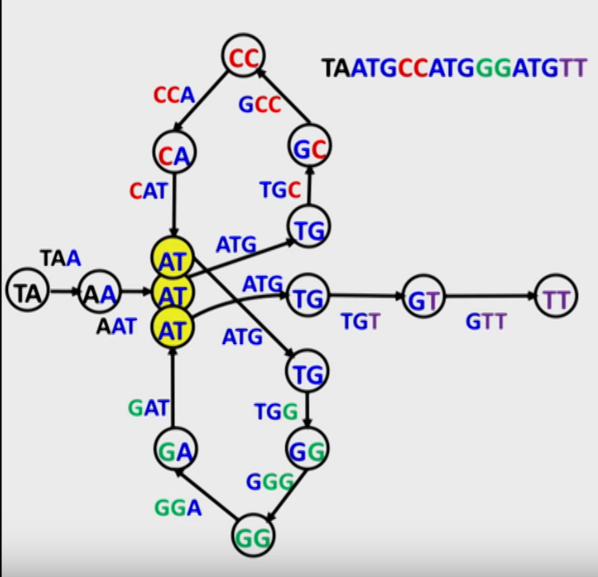
\includegraphics[scale = 0.4]{gluing2.png}
\end{figure}
\end{frame}

%------------------------------------------------

\begin{frame}
\frametitle{Collapsing like vertices on itself}
\begin{figure}[h]
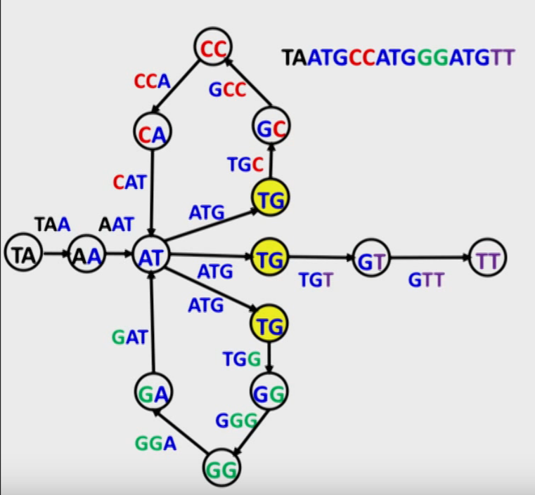
\includegraphics[scale = 0.4]{gluing3.png}
\end{figure}
\end{frame}

%------------------------------------------------

\begin{frame}
\frametitle{DeBruijn Graph of TAATGCCATGGGATGTT}
\begin{figure}[h]
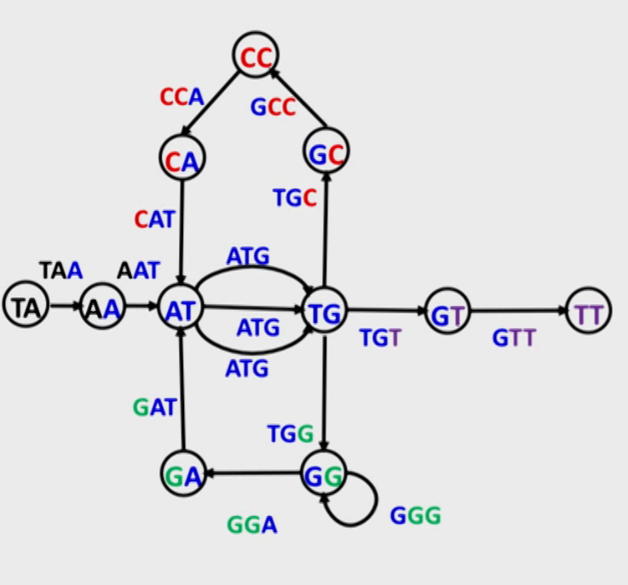
\includegraphics[scale = 0.4]{gluingfinal.png}
\end{figure}
\end{frame}

%------------------------------------------------

\begin{frame}
\frametitle{Reconstruction of TAATGCCATGGGATGTT}
\begin{itemize}
\item An Euler path on this digraph successfully constructs the genome that we are interested in. Of course for the demonstration purposes we started with the genome itself, but in reality all we have are partial reads
\pause
\item Debruijn graph holds the same data as the given genome does!
\pause
\item What if there are multiple Euler paths?
\pause
\item That is where we use paired Debruijn graphs (A special form of 4-mer and 6-mer pairing)
\end{itemize}
\end{frame}

%------------------------------------------------

\begin{frame}
\frametitle{References}
\footnotesize{
\begin{thebibliography}{99} % Beamer does not support BibTeX so references must be inserted manually as below
\bibitem[Smith, 2012]{p1} John Smith (2012)
\newblock Title of the publication
\newblock \emph{Journal Name} 12(3), 45 -- 678.
\end{thebibliography}
}
\end{frame}

%------------------------------------------------

\begin{frame}
\Huge{\centerline{The End}}
\end{frame}

%----------------------------------------------------------------------------------------

\end{document}